% Template for ICIP-2013 paper; to be used with:
%          spconf.sty  - ICASSP/ICIP LaTeX style file, and
%          IEEEbib.bst - IEEE bibliography style file.
% --------------------------------------------------------------------------
\documentclass{article}
\usepackage{spconf,amsmath,graphicx}

% Example definitions.
% --------------------
\def\x{{\mathbf x}}
\def\L{{\cal L}}

% Title.
% ------
\title{Parallel Training of Deep Neural Network using Model Averaging and Butterfly Mixing}
%
% Single address.
% ---------------
\name{Hang Su$^{1,2}$, Haoyu Chen$^1$, Haihua Xu$^3$}
\address{$^1$ International Computer Science Institute, Berkeley, California, US \\
$^2$ Dept. of Electrical Engineering \& Computer Science, University of California, Berkeley, CA, USA \\
$^3$ Nanyang Technological University, Singapore \\
{\small \tt \{suhang3240@gmail.com\}}
}
%
% For example:
% ------------
%\address{School\\
%	Department\\
%	Address}
%
% Two addresses (uncomment and modify for two-address case).
% ----------------------------------------------------------
%\twoauthors
%  {A. Author-one, B. Author-two\sthanks{Thanks to XYZ agency for funding.}}
%	{School A-B\\
%	Department A-B\\
%	Address A-B}
%  {C. Author-three, D. Author-four\sthanks{The fourth author performed the work
%	while at ...}}
%	{School C-D\\
%	Department C-D\\
%	Address C-D}
%
\begin{document}
%\ninept
%
\maketitle
%
\begin{abstract}
In this paper we apply model averaging and butterfly mixing to parallel training of deep neural network (DNN). 
Parallelization is done in a model averaging manner. Data is partitioned and distributed to different nodes for 
local model updates, and model averaging (reduce) is done every few minibatches. 

We use multiple GPUs for data parallelization, and Message Passing Interface (MPI) for communication between nodes. 
We investigate the effectiveness of Natrual Gradient for Stochasitc Gradient Descent (NG-SGD) in the model averaging
framework, and compare two learning rate schedule strategies for model update. We show that combination of 
NG-SGD and exponential learning rate schedule can lead to better convergence. On the 300h Swithboard dataset, a 10 
times speed up is achieved using 16 gpus with little decoding accuracy loss -- a 0.2\% degradation in word error rate 
(WER). We also introduce a butterfly mixing strategy that can further save communication costs in model averaging framework.
\end{abstract}
%
\begin{keywords}
Parallel training, model averaging, deep neural network, butterfly mixing
\end{keywords}
%
\section{Introduction}
\label{sec:intro}
Deep Neural Networks (DNN) has shown its effeciveness in several machine learning tasks, espencially in speech
recognition. The large model size and massive training examples make DNN a powerful model for classification. However,
these two factors also slow down the training procedure of DNNs.

Parallelization of DNN training has been a popular topic since the revival of neural networks. Several different strategies
have been proposed to tackle this problem. Multiple thread CPU parallelization and single GPU implementation are compared
in \cite{scanzio2010parallel,vesely2010parallel}, and it is shown that single GPU could beat multi-threaded CPU implementation
by a factor of 2.

Optimality for parallelization of DNN training was analyzed in \cite{seide2014parallelizability}, and based on the analysis, 
a gradient quantization approach (1-bit SGD) was proposed to minimize communication cost \cite{seide20141}. It shows that 1 bit
can effectively reduce the amount of data exchanged in an MPI framework, and a 10 times speed-up using 40 GPUs.

DistBelief proposed in \cite{dean2012large} reports that 8 CPU machines train 2.2 times faster than a single GPU machine on a
moderately sized speech model. Asynchronous SGD using multiple GPUs achieved a 3.2x speed-up on 4 GPUs \cite{zhang2013asynchronous}.

A pipeline training approach was propoased in \cite{chen2012pipelined} and a 3.3x speedup was achieved using 4 GPUs, but this
method does not scale beyond number of layers in the neural network.

A speedup of 6x to 14x was achieved using 16 GPUs on training convolutional neural networks \cite{coates2013deep}. In this approach,
each GPU is responsible for a partition of the neural network. This approach is more useful for image classification where 
local structure of the neural network could be exploited. For a fully connected speech model, a model partition approach 
may not be able to contribute as much.

Distributed model averaging using CPUs is proposed in \cite{zhang2014improving}, and a further improvement 
is done using natural gradient \cite{povey2014parallel}. In this approach, separate models are trained on multiple nodes using 
different partitions of data, and model parameters are averaged after each epoch. It is shown that NG-SGD can effectively improve
convergence and ensure a better model trained using the model averaging framework.

Our approach is mainly based on the NG-SGD with model averaging. The main differences here in this work are:
1. We utilize multiple GPUs in neural networks training via MPI, which allows us to perform model averaging more frequently and efficiently;
2. We introduce a butterfly-mixing strategy for model averaging that can further speed up the training.

In addition, this work simplifies the model training procedure in the following aspects:
1. It does not require a warm-up phase where only single thread can be used for model update \cite{seide20141,povey2014parallel};
2. It does not need to tune minibatch size to utilize parallelization power;
3. It does not use momentum or Adagrad\cite{duchi2011adaptive} for gradient estimation.

On the other hand, it requires:
1. A proper implementation of NG-SGD, as is introduced in \cite{povey2014parallel};
2. A bigger initial learning rate and a proper model averaging frequency;

In Section 2 we introduce the model averaging approach. In Section 3 we introduce butterfly-mixing strategie. Section 4 
explains NG-SGD. Section 5 records experimental results on different setups and Section 6 concludes.

\section{Data parallelization and Model Averging}
Stochastic gradient descent is a popular method for DNN training, even though this is a non-convex optimization 
problem. Since the size of training data is large, minibatch based SGD is often used for model training. 
Roughly, the larger the minibatch size, the higher the converge rate. However, a large minibatch requires
more compute and memory usage, so a straight forward idea for parallelization would be distributing the 
gradient computation to different computing nodes. In each step, the gradient is reduced to one computing node,
averaged and then used to update models in each node. This method can compute the gradient accurately, but 
it requires heavy communication between nodes.

However, if we choose to reduce the weight rather than gradient, it is not necessary to communicate that often. There
is straight forward theory that guarantees convergence, but we do observe reasonable results in experiments.


\section{Model Averaging Strategy}
\subsection{All-reduce}
All-reduce strategy collects the weights from all the nodes in the network. The communication is bounded by 
the bandwidth. Fig~\ref{fig:allreduce} is an example of all-reduce with 4 nodes. One node is responsible for
collecting all the model parameters. It will average the weights and then broadcast it to all the nodes. 
This approach compute the average weight based on all the information in computing nodes. Thus, we expect 
the converge speed to be the fastest.
\begin{figure}[htb]
  \centering
  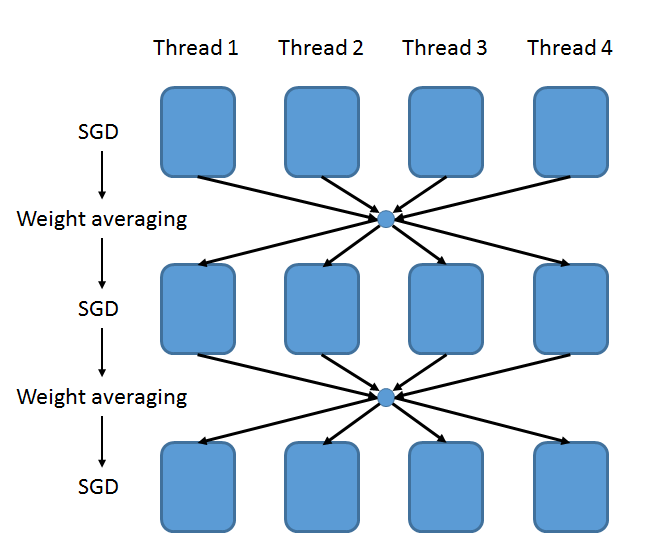
\includegraphics[width=0.5\textwidth]{allreduce.png}
  \caption{All-reduce network}
  \label{fig:allreduce}
\end{figure}

\subsection{Butterfly mixing}
Butterfly mixing was proposed in \cite{zhao2013butterfly} to interleave communication with computation. In each
reduce period, information (gradient / model) is exchanged between each node and its friend node. The pair of nodes
are shuffled after every reduce so that information in each node can propagate to all other nodes in $log(numNodes)$ periods.


Butterfly mixing is a reduction strategy proposed in \cite{zhao2013butterfly}. It reduces the communication load in 
every iteration: one node would only send and receive message from one other node. The pairing of nodes are shuffled after
each reduction so that information collected in each nodes will spread to all other nodes. Fig~\ref{fig:butterfly} 
is an example of butterfly mixing with 4 nodes. Butterfly mixing requires much less communication than all-reduce 
strategy. However, each node in the network only collects information from two computing nodes at a time.
It takes $log(numNodes)$ communication to spread the message to the whole network. Thus, the converge speed 
of butterfly mixing would be slower than all-reduce strategy. 
\begin{figure}[htb]
  \centering
  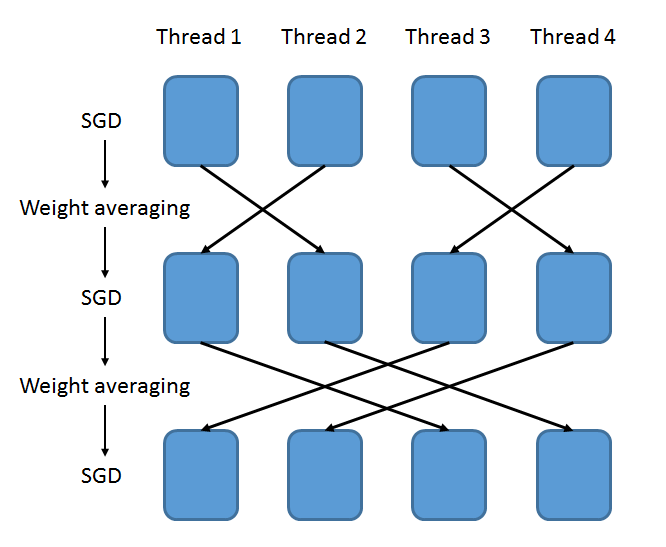
\includegraphics[width=0.5\textwidth]{butterfly.png}
  \caption{Butterfly mixing network}
  \label{fig:butterfly}
\end{figure}

\subsection{Data exchange analysis}

\section{Natural Gradient for Model Update}
In stochastic gradient descent (SGD), the learning rate is often assumed to be a scalar $\alpha_t$ that may change over time,
the update formula for model parameters $\theta_{t}$ is
\begin{equation}
\theta_{t+1} = \theta_{t} + \alpha_t g_t
\end{equation}
where $g_t$ is the gradient.

However, according to Natural Gradient idea \cite{murata1999statistical,roux2008topmoumoute}, it is possible to replace 
the scalar with a symmetric positive definite matrix $E_t$, which is the inverse of the Fisher information matrix.
\begin{equation}
\theta_{t+1} = \theta_{t} + \alpha_t E_t g_t
\end{equation}

Suppose $x$ is the variable we are modeling, and $f(x;\theta)$ is the probability or likelihood of $x$ given parameters $\theta$, then the
Fisher information matrix $I(\theta)$ is defined as
\begin{equation}
\frac{\partial}{\partial\theta}\log f(x;\theta)
\end{equation}

For large scale speech recognition, it is impossible to estimate Fisher information matrix and perform inversion, 
so it is necessary to approximate the inverse Fisher information matrix directly. We do not include too much 
detail here because this is not the main focus of this report. Details about implementation of NG-SGD could 
be found in \cite{povey2014parallel}.

\section{Initialization}
Conjecture: dbn pretraining initialize the neural network such that it lies in a convex-like area

\section{Experimental Results}
\subsection{Setup}

\subsection{Learing Rate Schedule}


\subsection{Switchboard}

scaling factor
\begin{figure}[htb]
  \centering
  \includegraphics[width=0.5\textwidth]{scaling.png}
  \caption{Scaling factor and speedup factor v.s. number of gpus}
  \label{fig:scaling}
\end{figure}

percentage of time spent on communication
\begin{figure}[htb]
  \centering
  \includegraphics[width=0.5\textwidth]{percent.png}
  \caption{Percentage of time on MPI communication v.s. number of gpus}
  \label{fig:percent}
\end{figure}

\begin{table}
  \centering
  \begin{tabular}{c|c|c|c|c|c}
    \hline
     Nodes  & 1    & 2    & 4    & 8    & 16 \\
    \hline
Allreduce &    14.9 & -- & -- & 15.1 & 15.1 \\
    \hline
Butterfly &    14.9 & -- & -- & -- & --\\
    \hline
  \end{tabular}
  \caption{Comparison of WERs using different number of GPUs }
  \label{tab:wer}
\end{table}


\section{Conclusion and Future Work}
Neural network training can be efficiently speed up by using model averaging techniques and NG-SGD. 
Butterfly-mixing and ring reduction can reduce communication time a lot, but the models may not converge as well as 
Allreduce when the number of jobs goes up to 16.


CUDA aware MPI, learning rate schedule.


\section{Acknowledgements}
We would like to thank Karel Vesely and Daniel Povey who wrote the original "nnet1" neural network training code
and natural gradient stochastic gradient descent upon which the work here is based. We would also like to thank Nelson 
Morgan, Forrest Iandola and Yuansi Chen for their helpful suggestions.

% References should be produced using the bibtex program from suitable
% BiBTeX files (here: strings, refs, manuals). The IEEEbib.bst bibliography
% style file from IEEE produces unsorted bibliography list.
% -------------------------------------------------------------------------
\bibliographystyle{IEEEbib}
\bibliography{paper}

\end{document}
